\documentclass[12pt,english]{article}
\usepackage{lmodern}
	\renewcommand{\sfdefault}{lmss}
	\renewcommand{\ttdefault}{lmtt}
	\renewcommand{\familydefault}{\rmdefault}
\usepackage[T1]{fontenc}
\usepackage[latin9]{inputenc}
\usepackage{geometry}
	\geometry{verbose,tmargin=3cm,bmargin=3cm,lmargin=3cm,rmargin=3cm}
	\setcounter{secnumdepth}{-1}
\usepackage{fancyhdr}
\usepackage{color}
\usepackage{babel}
\usepackage{array}
\usepackage{float}
\usepackage{graphicx}
\usepackage{setspace}
\usepackage[unicode=true, bookmarks=true, bookmarksnumbered=false, bookmarksopen=false, breaklinks=false, pdfborder={0 0 1}, backref=section,colorlinks=true]{hyperref}
\hypersetup{pdfauthor={Max Stillwell}{Jacob Flynn}{Sasha Solomon}, pdfkeywords={BFF}{Bassoon Fingering Finder}, unicode=false, pdftoolbar=true, pdfmenubar=true, pdfstartview={FitV}, pdfnewwindow=true, linkcolor=blue, citecolor=blue, filecolor=blue, urlcolor=blue}

\pagenumbering{roman}
\makeatletter
	\providecommand{\tabularnewline}{\\}
	\@ifundefined{definecolor}{\usepackage{color}}{}
	\usepackage{lastpage}
	\renewcommand{\thepart}{}
	\renewcommand{\thesection}{}
	\renewcommand{\thesubsection}{}
\makeatother

\fancyhf{}
	\headheight 14.49998pt
	\pagestyle{fancy}
	\rhead{Bassoon Fingering Finder}
	\lfoot{\thepage}
	\cfoot{of}
	\rfoot{\pageref{LastPage}}

\onehalfspacing
%\setlength{\parindent}{0.0cm} %Uncomment to remove paragraph indents.

\begin{document}
\title{Bassoon Fingering Finder}
\author{Jacob Flynn, Sasha Solomon, Max Stillwell}
\maketitle
\begin{center}
	\begin{figure}
		\begin{centering}
			
\includegraphics{bff_logo1_small}
			\par
		\end{centering}
	\end{figure}
	\par
\end{center}
\pagebreak{}

\tableofcontents{}\clearpage{}

\setcounter{page}{1}
\pagenumbering{arabic}

\section{Executive Summary}
We designed a web application that helps bassoonists of all skill
levels find and learn new fingerings with an easy to use interface.

Bassoon fingerings can be very difficult to learn, especially because
there can be multiple fingerings for one note. Beginners and professionals
alike have the need to lookup fingerings for a note, usually in a
specific passage, to be sure they are using the appropriate fingering.
Bassoonists need to be able to access this tool via a personal computer,
a tablet (iPad, etc.), or smart-phone (Android, iPhone, etc.), and
would need to be able to easily search for fingerings for a specific
note. They also need to be able to add new fingerings, edit and delete
fingerings, and 'like'/'dislike' fingerings, as well as view fingerings
based on skill level.

This application will be beneficial to many bassoonists because it
gives them an easy way to find fingerings for specific notes based
on their skill level. It also gives bassoonists a social medium for
sharing fingerings, as well as suggestions and preferences for certain
fingerings.

\section{Background}
\subsection{Motivation}
The Bassoon Fingering Finder Team is very interested in evolutionary
computation and artificial intelligence, as well as mobile applications.
This project will not only help bassoonists, but also allowed the
BFF team to explore methods for using evolutionary computation and
artificial intelligence in a full software project. Also, because
the application needed to be compatible across multiple platforms,
it also gave the team experience with compatibility and mobile applications.

\subsection{Need}
Currently bassoonists have very few options when it comes to finding
fingerings quickly (which many times imperative during a concert or
recital). There are books listing hundreds of standard fingerings,
as well as an mobile fingering application with limited capabilities.
Bassoonists need a way to access fingerings quickly and be able to
search for fingerings they need. Also, because bassoonists have no
social medium for discussing preferences or suggestions for fingerings,
or receiving help for certain fingerings, it would also be helpful
to have an application that not only helped bassoonists find fingerings,
but also allowed them to communicate with fellow bassoonists.

\subsection{Benefits}
This project will benefit bassoonists, from beginners to professionals,
and will provide a way for bassoonists to communicate through a bassoon
specific application. Bassoonists will be able to add, edit, delete,
view, and search for bassoon fingerings with an easy to use graphical
interface, as well as manage fingerings they have added, 'like'/'dislike'
fingerings, and access the application via personal computer or mobile
devices.

\section{Problem Definition}
\subsection{Goals and Deliverables}
Create an interactive web application that would include 
\begin{itemize}
\item fingerings add/edit/delete/view/search 
\item sources for fingerings 
\item examples in literature 
\item comments 
\item likes/dislikes 
\item a graphical user interface that makes it easy to enter in fingerings 
\item accessibility via mobile devices as well as personal computers 
\item users that must login to be able to add/edit/delete fingerings 
\end{itemize}

\subsection{Specifications and Constraints}
\begin{itemize}
\item Ruby v. 1.9.3 
\item Rails web framework v. 3.2.0 
\item Postgres database v. 9.1.3 
\item Hosted through Heroku 
\item Viewable via PC/tablet/smart-phone 
\item Supports Chrome/Firefox/Safari/Opera 
\end{itemize}

\section{Project Plan}
\subsection{Tasks and Schedule}
\begin{itemize}
\item First Infrastructure
\item Second Database
\item Third For users
\item Third For note/fingering combinations
\item Second Users
\item Third Authentication
\item Fourth Basic user
\item Fourth Administrative user
\item Third Email verification
\item Third Time zone specification
\item Third Skill level
\item First Web-page
\item Second Information organization
\item Second Professional appearance
\item First Application
\item Second Fingering chart
\item Second Scale for notes
\item Second Input of a note
\item Second Input of a fingering
\item Second Store a note/fingering combination
\item Second Approve a note/fingering combination
\item Second Search a note for a list of associated fingerings
\item Second Sort list of associated fingerings by rating, based on skill level
\item Second Add a series of notes
\item Second Search a series of notes
\item Second Like/Dislike a note/fingering combination
\end{itemize}

\subsection{Team Responsibilities}
Jacob's primary task was the infrastructure.  He worked to get the user
authentication, time zone specification, and skill level functioning.
He setup the ability for users to be able to view and edit their 'profile'
information, containing their skill level, email address, ect.  Once those
tasks were done, he moved to work on bug reports and assist with the application
section when needed.

Sasha's primary task was

Max's primary task was the JavaScript, HTML5, \& CSS related parts. He mainly worked on the HTML5+JavaScript
canvas for the note/fingering entry, editing, and display. He also worked on the browser side validation JavaScripts for
the various forms on the website. He worked on adapting a free CSS template for use on the site and added various CSS
rules for things like tabs and tables. Lastly he handled filtering most bug reports to their respective developers, i.e. filtering user
bugs to Jacob and search bugs to Sasha.

\section{Concepts Considered}
\subsection{Implementation Model: Web application vs. Fully Mobile}
Though the project proposal suggested the model be implemented via
a web application, our sponsor voiced the need to have the application
be functional on mobile devices as well. Though it would be an interesting
opportunity to build a fully mobile application, the team had no experience
with building mobile applications.

\subsection{Programming Language: Python/Django vs. Ruby/Rails}
Originally, we considered using python with the django web framework
to develop the application. Both languages are scripting languages
that lend themselves to web development. All members of the team had
experience working with Python and Django previously on the software
engineering project for CS383/384. However, Ruby/Rails is ubiquitous
in web development currently and would be an opportunity to learn
a new language and web framework.

\subsection{Applet Language: Java vs. Flash vs. JavaScript+HTML5}
Java and flash are both often used in web development to build applets and therefore are
well supported on most modern PC browsers with up to date plugins. However, mobile browsers 
this is not the case with Java applets unable to run on Android and iPhone, and Flash only running 
on newer versions of the Android OS. JavaScript+HTML5 is fairly new but runs on any browser including
mobile devices albeit with varying levels of support for various features, and requires no extra plugins
to install and keep up to date.

\subsection{Validation Methods: In-house vs. Devise}
Because the application was fairly small and specific, the team decided
in-house validation may be easier and better suited to the application.
However, as the application continued to develop, it became a much
larger application than originally modeled. The validation plug-in,
Devise, provides built-in validation tools that are easy to integrate
with applications.

\subsection{Search Results Rating Algorithm: Ratio Rating vs. Confidence Interval Rating}
The simple rating algorithm involved finding the ratio of `likes'
and `dislikes' of a fingering (i.e. likes divided by likes plus dislikes).
However, this rating algorithm could possibly rate fingerings inappropriately.
For example, if fingering one had 100 likes and 50 dislikes, while
fingering two had 1 like and no dislikes, fingering 2 would be rated
higher than fingering one, even though fingering 1 should be rated
higher.

\section{Concept Selection}
\subsection{Implementation Model: Web application vs. Fully Mobile}
Because the sponsor still wanted a mobile application in addition
to a web application, the team decided to implement a mobile compatible
web application to cater to users of both PC's and mobile devices.

\subsection{Programming Language: Python/Django vs. Ruby/Rails}
However, the team decided that gaining experience working with Ruby
on Rails, which is ubiquitous in web application development, would
be prudent.

\subsection{Applet Language: Java vs. Flash vs. JavaScript+HTML5}
Since the application was to be mobile device compatible JavaScript+HTML5 was
chosen for the language of the applet that was to handle the entering, display, and
editing of bassoon key fingerings.

\subsection{Validation Methods: In-house vs. Devise}
However, after trying to implement Devise on partially implemented
application, it became apparent that the application was too far along
in development to gain use from Devise.

\subsection{Search Results Rating Algorithm: Ratio Rating vs. Confidence Interval Rating}
The team decided to use a more accurate rating algorithm that take
into account the volume of likes/dislikes and how well received the
fingering is (i.e. if it is `controversial'). The algorithm used is
as follows:

\[
(\hat{p}+z_{\frac{\alpha}{2}}^{2}\pm z_{\frac{\alpha}{2}}\sqrt{(\hat{p}(1-\hat{p})+z_{\frac{\alpha}{2}}^{2}/4n)/n})/(1+z_{\frac{\alpha}{2}}^{2}/n)
\]

\section{System Architecture}
\subsection{Conceptual Design}
Conceptually, the web application would be based on a Model-View-Controller
architecture.

\begin{figure}[H]
	\caption{MVC Architecture}
	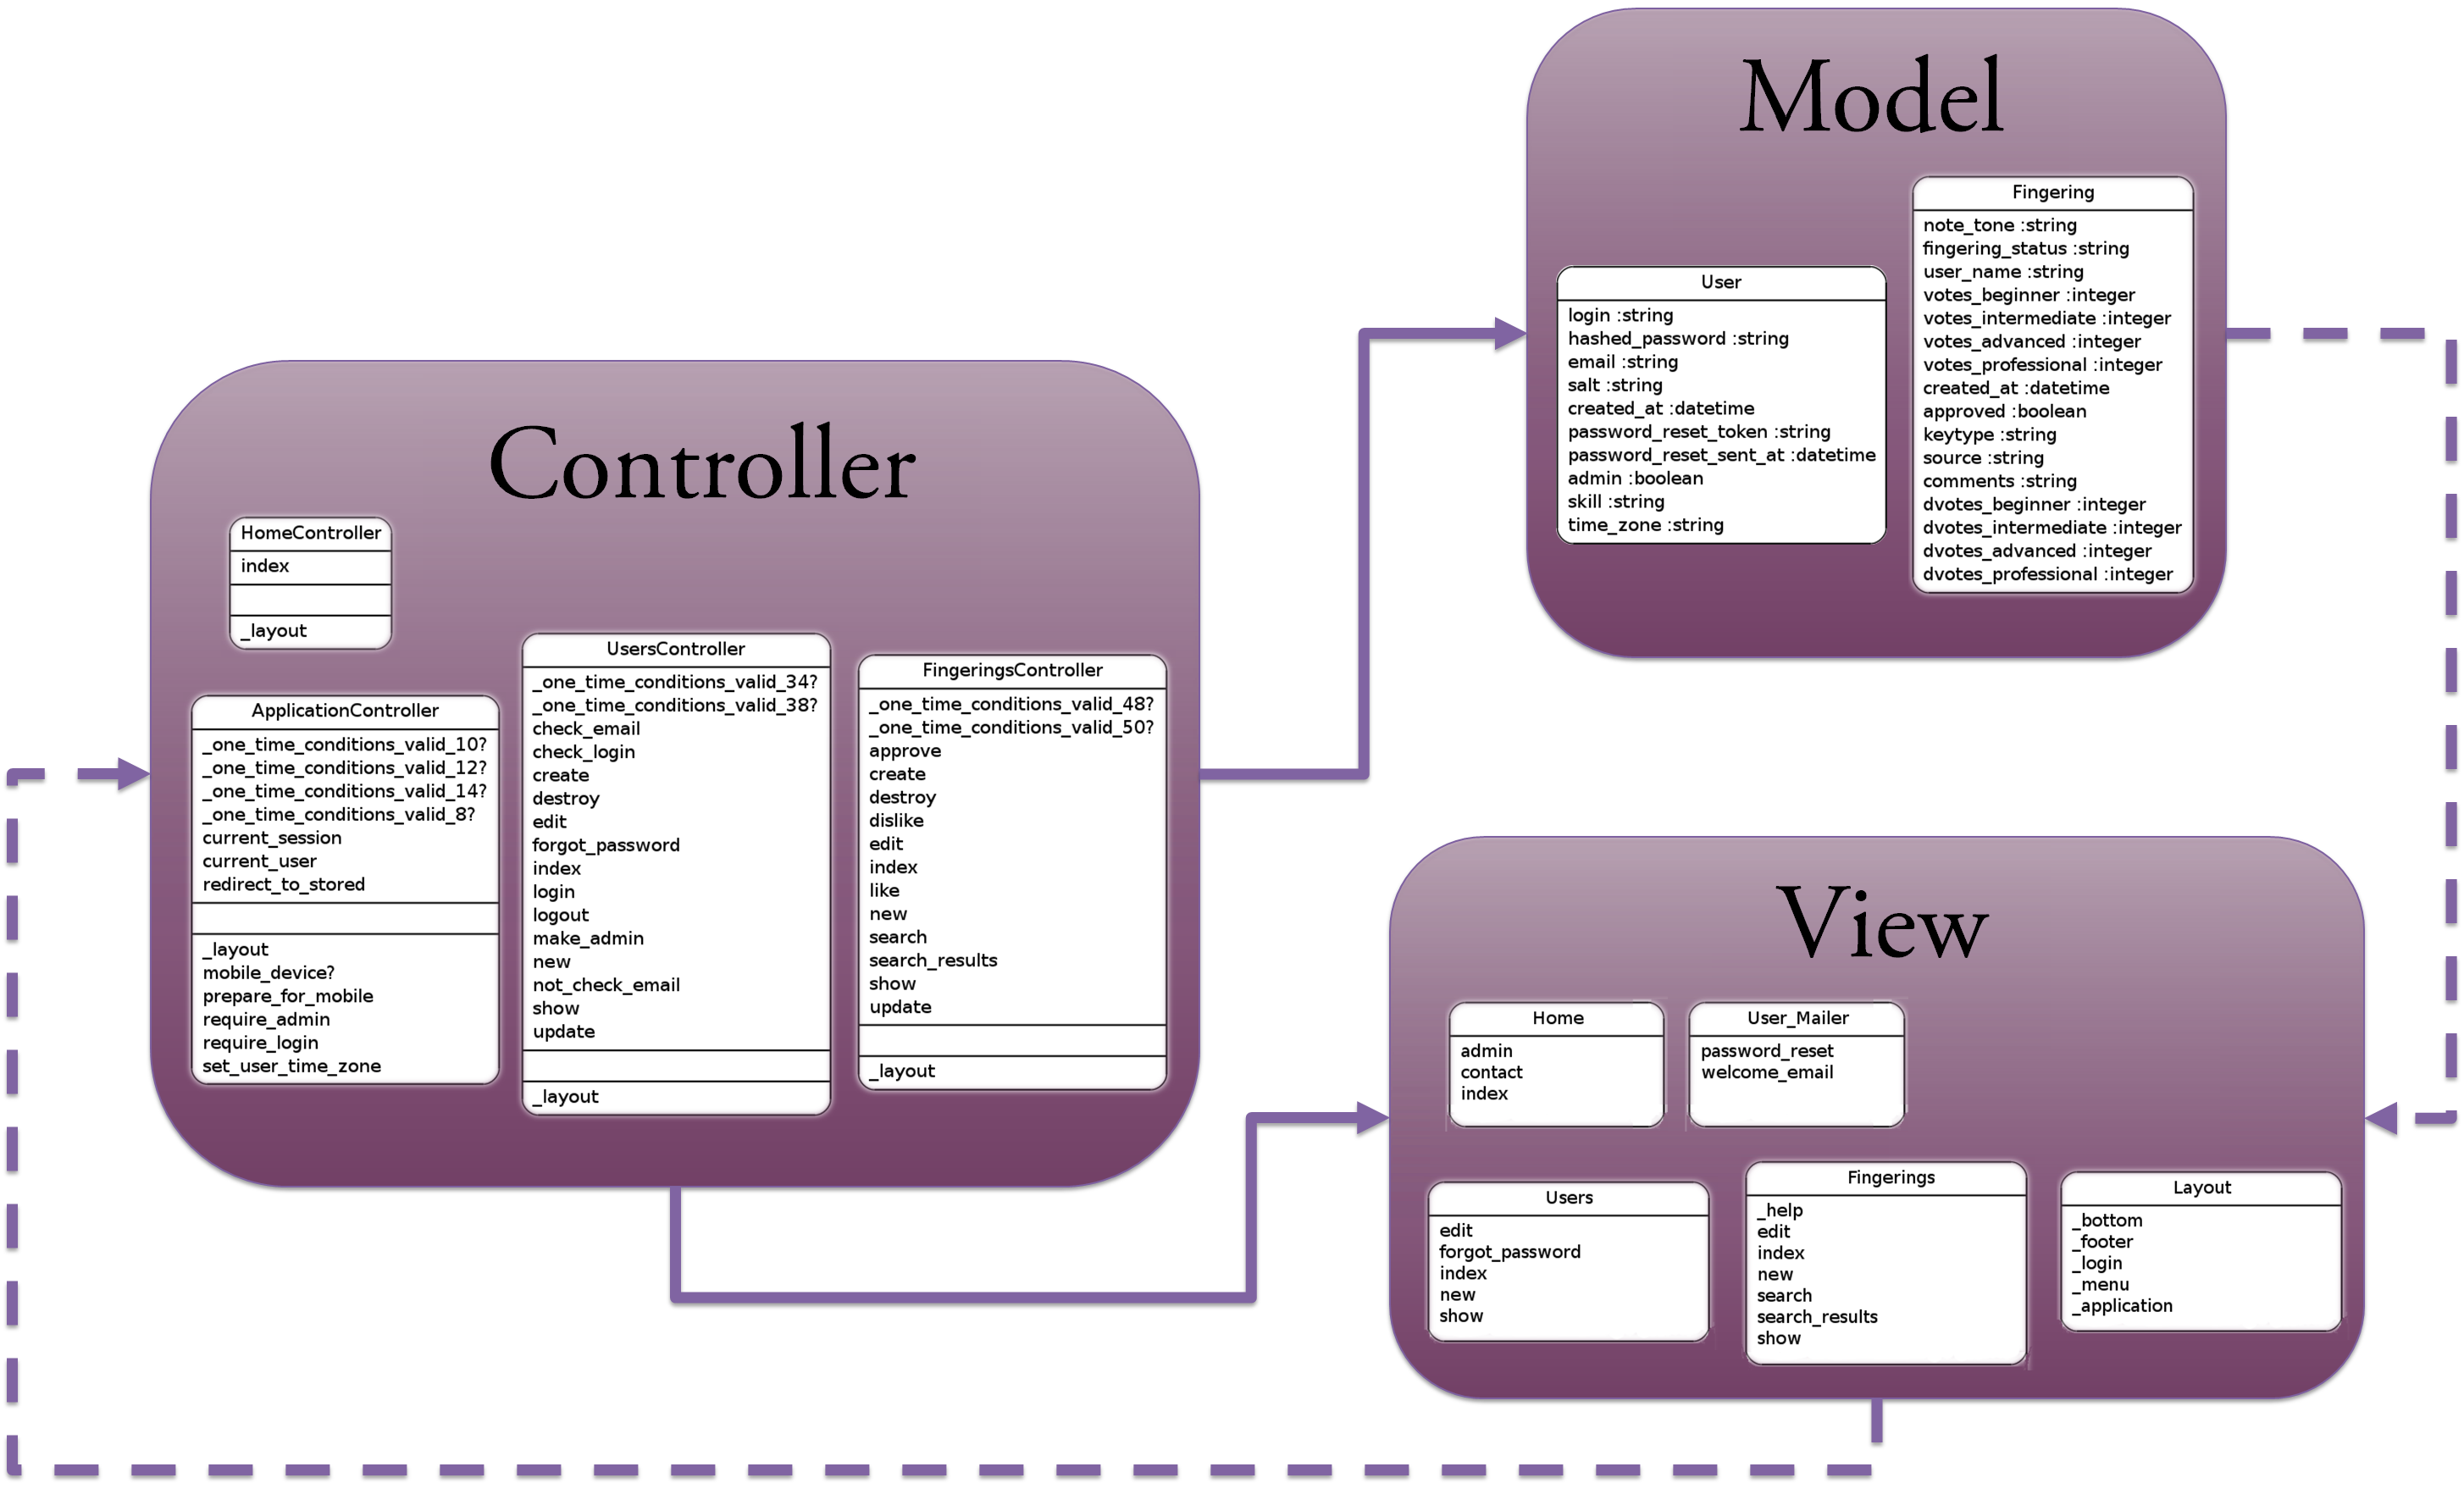
\includegraphics[scale=0.15]{MVC} 
\end{figure}

\subsection{Components and How Integrated}


\subsection{Results from Tests/Analysis}
The initial beta group, consisting primarily of our sponsor Dr. Susan Hess,
response was reasonably positive.  They submitted several bug reports, 
and a few feature requests but overall provided fairly positive feedback 
about the features that were functioning and fully implemented.

The response remained positive after we moved to a larger test group
including students and associates of our Dr. Hess.  While Dr. Hess continued
to be the primary tester, submitting the majority of bug reports and feature
requests, the other users did not mention any major concerns about the application.

We were also able to get some feedback during the Engineering EXPO.  This
was also fairly positive.  One of the biggest questions was if we could, or
if we planned, on expanding the application to other instruments.  We also
had a number of non-bassoon players take a look at the application and while
they were initially confused about the layout of the fingering chart, they
appreciated the application for the problem it solves.

\section{Future Work}
Work for this project is intended to continue next semester in order
to implement the current application on a mobile platform. Though
the current web application is usable via mobile browsers, a mobile
application would provide the flexibility and flow specific to mobile
devices.

In addition to a mobile version, the web application version would
be continued to include features available in the premium version
of the web application. These premium features would include, but
is not limited to the following:

\begin{enumerate}
	\item Being able to hear the sound of each note as it is selected. 
	\item Searching more than just standard fingerings, (i.e. the fingerings
		searchable on the site will only be basic, and in order to view many
		alternate fingerings one would have to pay for the app) 
	\item A mobile optimized version of the site. 
	\item Input of multiple fingering/note combinations. 
	\item Searching of a fingering to find the note associated, in addition
		to searching the note for the fingerings. 
\end{enumerate}

The implementation of a mobile application, as well as a premium web
application, would require a full semester to complete and could be
implemented by a future Computer Science Senior Design Team.
\clearpage

\section{Appendices}
\subsection{Software Requirements}
\begin{tabular}{|p{3cm}|p{13cm}|}
	\hline 
	\multicolumn{2}{|l|}{\textbf{Web Browsers}}\tabularnewline
	\hline 
	\textbf{Description}  & Be viewable on most web browsers including mobile web browsers. \tabularnewline
	\hline 
	\textbf{Notes}  & 
		\begin{itemize}
			\item None.
		\end{itemize}
	\tabularnewline
	\hline 
\end{tabular}\\[0.5cm]

\subsection{Application Requirements}
\begin{tabular}{|p{3cm}|p{13cm}|}
	\hline 
	\multicolumn{2}{|l|}{\textbf{Show Fingering/Note Combinations}}\tabularnewline
	\hline 
	\textbf{Description}  & Show a fingering combination for a note or a series of notes. \tabularnewline
	\hline 
	\textbf{Notes}  & 
		\begin{itemize}
			\item None.
		\end{itemize}
	\tabularnewline
	\hline 
\end{tabular}\\[0.5cm] %
\begin{tabular}{|p{3cm}|p{13cm}|}
	\hline 
	\multicolumn{2}{|l|}{\textbf{Enter Fingering/Note Combinations}}\tabularnewline
	\hline 
	\textbf{Description}  & Ability to add new fingering/note combinations. \tabularnewline
	\hline 
	\textbf{Notes}  & 
		\begin{itemize}
			\item None. 
		\end{itemize}
	\tabularnewline
	\hline 
\end{tabular}\\[0.5cm] %
\begin{tabular}{|p{3cm}|p{13cm}|}
	\hline 
	\multicolumn{2}{|l|}{\textbf{Edit Fingering/Note Combinations}}\tabularnewline
	\hline 
	\textbf{Description}  & Ability to edit existing fingering/note combinations. \tabularnewline
	\hline 
	\textbf{Notes}  & 
		\begin{itemize}
			\item None. 
		\end{itemize}
	\tabularnewline
	\hline 
\end{tabular}\\[0.5cm] %
\begin{tabular}{|p{3cm}|p{13cm}|}
	\hline 
	\multicolumn{2}{|l|}{\textbf{Remove Fingering/Note Combinations}}\tabularnewline
	\hline 
	\textbf{Description}  & Ability to remove existing fingering/note combinations. \tabularnewline
	\hline 
	\textbf{Notes}  & 
		\begin{itemize}
			\item None. 
		\end{itemize}
	\tabularnewline
	\hline 
\end{tabular}\\[0.5cm]

\subsection{User Requirements}
\begin{tabular}{|p{3cm}|p{13cm}|}
	\hline 
	\multicolumn{2}{|l|}{\textbf{Fingering Request for Notes}}\tabularnewline
	\hline 
	\textbf{Description}  & Ability to select a series of up to three fingerings and request a
		fingering progression for those notes. \tabularnewline
	\hline 
	\textbf{Notes}  & 
		\begin{itemize}
			\item Can request alternate fingerings. 
			\item Can view example music for the fingerings. 
			\item Can sort fingerings by hole coverage or expertise level. 
			\item Can \textquotedbl{}Like\textquotedbl{} or \textquotedbl{}Dislike\textquotedbl{}
				the given fingerings. (Requires Login) 
			\item Can submit a new fingering for the chosen note progression. (Requires Login) 
			\begin{itemize}
				\item Can attach example music to the new fingering. (Requires Login) 
				\item Can set the expertise level of the new fingering. (Requires Login)
			\end{itemize}
		\end{itemize}
	\tabularnewline
	\hline 
\end{tabular}\\[0.5cm]

\subsection{Administrative User Requirements}
\begin{tabular}{|p{3cm}|p{13cm}|}
	\hline 
	\multicolumn{2}{|l|}{\textbf{Add New Fingering}}\tabularnewline
	\hline 
	\textbf{Description}  & Ability to add a new fingering for a given set of notes. (Requires Login) \tabularnewline
	\hline 
	\textbf{Notes}  & 
		\begin{itemize}
			\item None 
		\end{itemize}
	\tabularnewline
	\hline 
\end{tabular}\\[0.5cm] %
\begin{tabular}{|p{3cm}|p{13cm}|}
	\hline 
	\multicolumn{2}{|l|}{\textbf{Remove Existing Fingering}}\tabularnewline
	\hline 
	\textbf{Description}  & Ability to remove a new fingering from the database. (Requires Login) \tabularnewline
	\hline 
	\textbf{Notes}  & 
		\begin{itemize}
			\item None 
		\end{itemize}
	\tabularnewline
	\hline 
\end{tabular}\\[0.5cm] %
\begin{tabular}{|p{3cm}|p{13cm}|}
	\hline 
	\multicolumn{2}{|l|}{\textbf{Update Fingering}}\tabularnewline
	\hline 
	\textbf{Description}  & Ability to update and existing fingering in the database. (Requires Login) \tabularnewline
	\hline 
	\textbf{Notes}  & 
		\begin{itemize}
			\item None. 
		\end{itemize}
	\tabularnewline
	\hline 
\end{tabular}\\[0.5cm] %
\begin{tabular}{|p{3cm}|p{13cm}|}
	\hline 
	\multicolumn{2}{|l|}{\textbf{Approve User Added Fingering}}\tabularnewline
	\hline 
	\textbf{Description}  & Approve a fingering added by a user for use in the database. (Requires Login) \tabularnewline
	\hline 
	\textbf{Notes}  & 
		\begin{itemize}
			\item None. 
		\end{itemize}
	\tabularnewline
	\hline 
\end{tabular}\\[0.5cm] %
\begin{tabular}{|p{3cm}|p{13cm}|}
	\hline 
	\multicolumn{2}{|l|}{\textbf{Deny User Added Fingering}}\tabularnewline
	\hline 
	\textbf{Description}  & Deny a fingering added by a user. (Requires Login) \tabularnewline
	\hline 
	\textbf{Notes}  & 
		\begin{itemize}
			\item None. 
		\end{itemize}
	\tabularnewline
	\hline 
\end{tabular}\\[0.5cm] %
\begin{tabular}{|p{3cm}|p{13cm}|}
	\hline 
	\multicolumn{2}{|l|}{\textbf{Freeze User Like/Dislike Options}}\tabularnewline
	\hline 
	\textbf{Description}  & Ability to prevent users from Like/Disliking specific fingerings or all 
		fingerings. (Requires Login) \tabularnewline
	\hline 
	\textbf{Notes}  & 
		\begin{itemize}
			\item None. 
		\end{itemize}
	\tabularnewline
	\hline 
\end{tabular}\\[0.5cm] %
\begin{tabular}{|p{3cm}|p{13cm}|}
	\hline 
	\multicolumn{2}{|l|}{\textbf{Unfreeze User Like/Dislike Options}}\tabularnewline
	\hline 
	\textbf{Description}  & Ability to allow users to Like/Dislike specific fingerings or all
		fingerings. (Requires Login) \tabularnewline
	\hline 
	\textbf{Notes}  & 
		\begin{itemize}
			\item None. 
		\end{itemize}
	\tabularnewline
	\hline 
\end{tabular}\\[0.5cm] 
\end{document}
